%!TEX root = ../thesis.tex
% User scenario using the DemoDraw system

\section{Creating Illustrations with DemoDraw}

\systemname{} is designed for non-experts who cannot effectively or efficiently create concise motion illustrations motions using existing tools.
To provide an overview of how the system works, we present a scenario in which a motion illustration author, Marie, creates instructions for an 8-step dance tutorial.

In her living room, Marie begins using \systemname{} with the \phaseI{} shown on her television by standing in front of a Kinect. In the center of the display, an avatar follows her movements in real-time (Figure~\ref{fig:DemoDrawUI}a).
This avatar is shown as an ``outline'' figure, but she could always change to different rendering effects like ``silhouette'' or ``cartoon,'' or select a different 3D human model later using our \phaseII{} (Figure~\ref{fig:DemoDrawRefinementUI}a).

\begin{figure*}[!t]
  \centering
  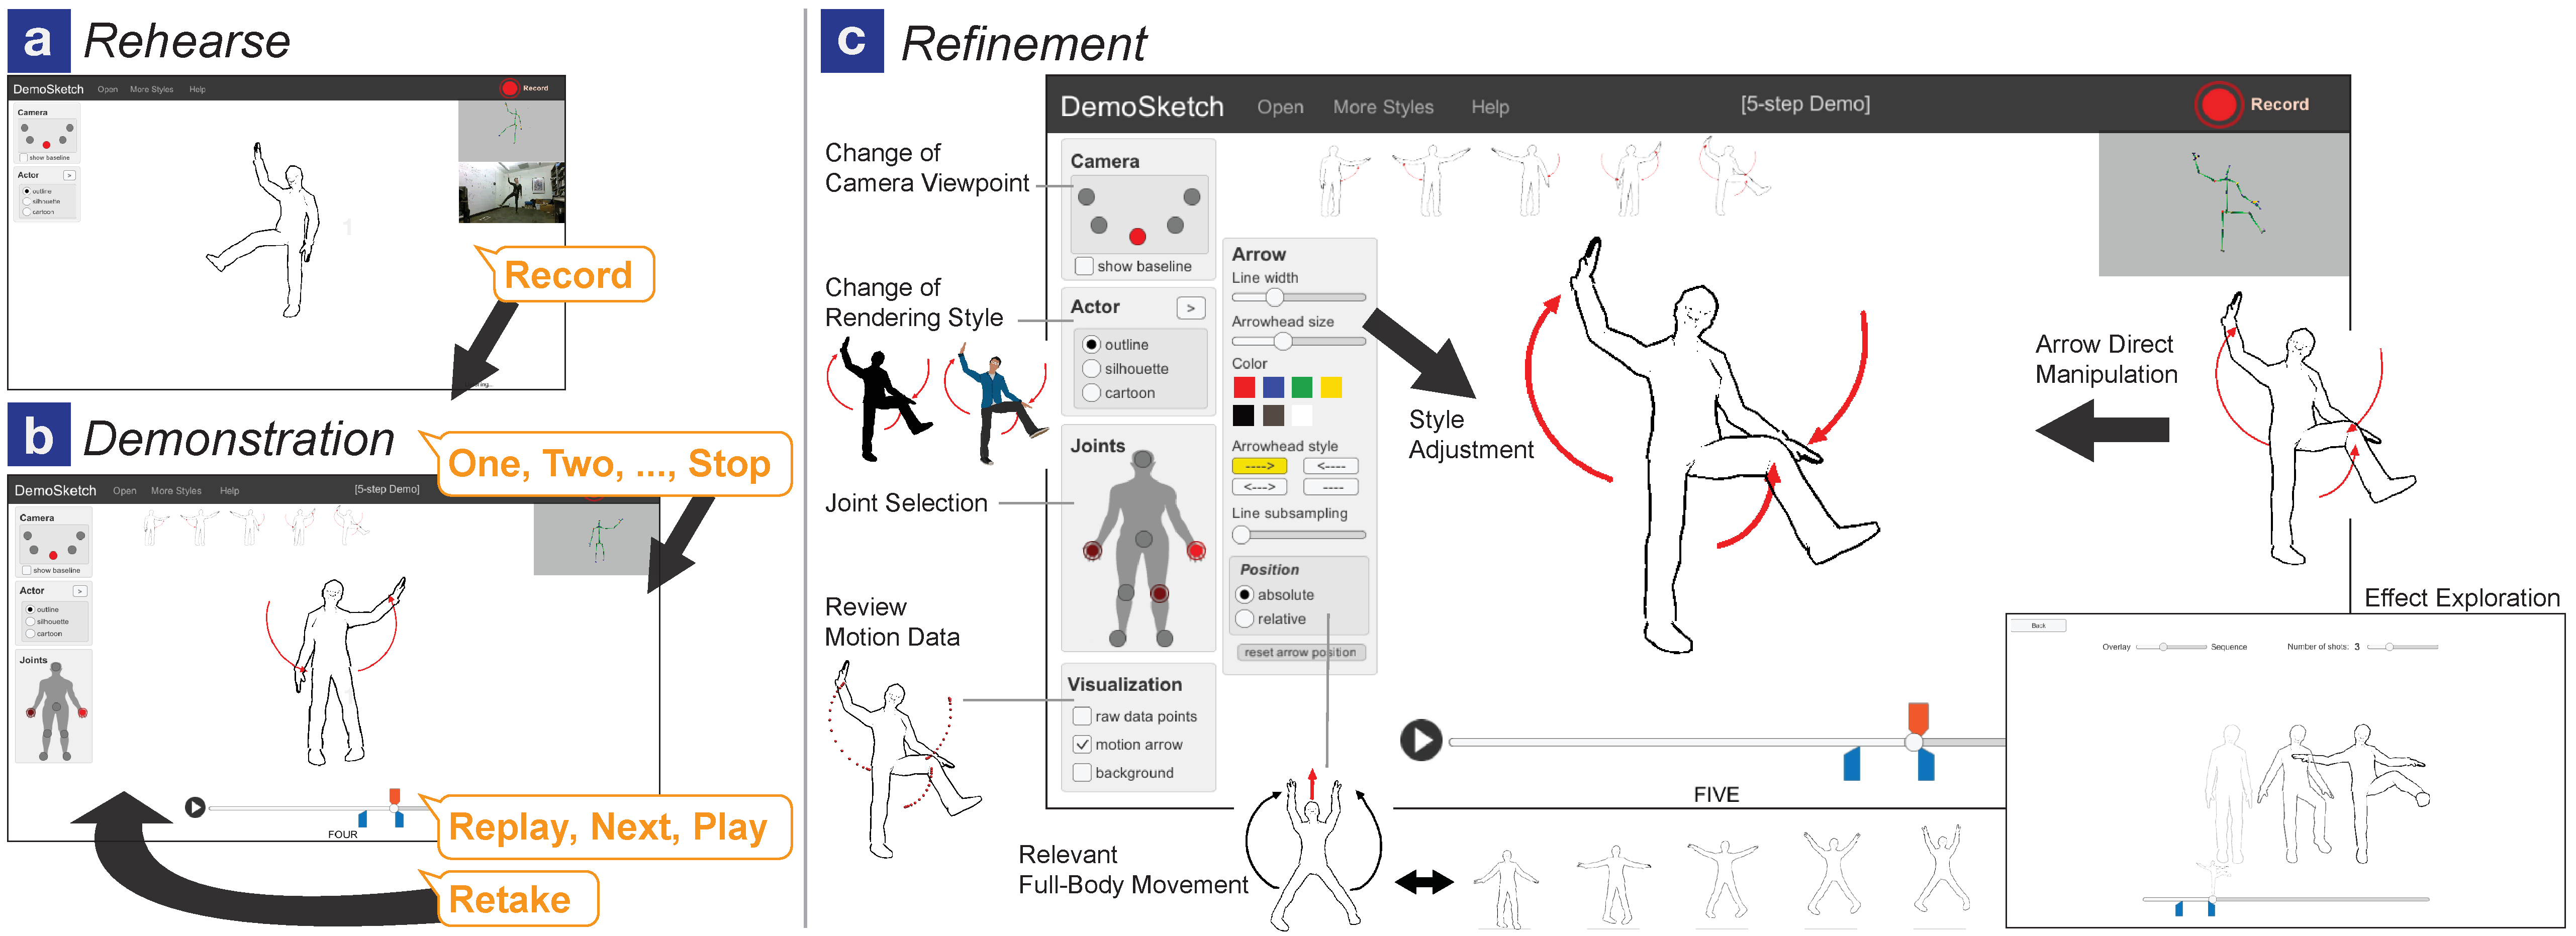
\includegraphics[width=0.75\textwidth]{\demodraw/fig/ui/ui}
  \caption{\systemname{} authoring UI: Using the \phaseI{}, an author sees an avatar following her real-time movement (a). During recording (initiated by voice command ``Start''), real-time feedback shows the speech labels (b). Once a recording is completed by voice command ``Stop'', the motion visualization and a timeline are immediately available (c) for the author to review, and a step-by-step overview will be generated.}
  \dan{I changed figure start command to Start to match the video.}
  \label{fig:DemoDrawUI}
\end{figure*}

\subsubTitleBold{Recording}
Marie starts recording her physical demonstration with the voice command \iquote{Start.} After a 3-second countdown, \systemname{} captures the position, orientation, and depth distance of her body (using Kinect's simplified 25 body joint model).
%
While demonstrating dance moves, Marie verbally indicates the count of each step with \iquote{one, two, three, and four,} just like she does when teaching a dance. The specific utterance is not constrained, Marie could use words like \iquote{right, left, shake, and clap.} A speech recognition engine captures these labels with timestamps and displays them in the interface (Figure~\ref{fig:DemoDrawUI}b).
Marie finishes recording by saying \iquote{Stop}.

\subsubTitleBold{Reviewing and Re-Recording}
After recording, \systemname{} automatically segments the motion around the speech labels and identifies salient joints. An illustration of the first step of Marie's demonstration is rendered with motion arrows, showing the path of the most salient joints. Figure~\ref{fig:DemoDrawUI}c presents an example illustration that shows how her right hand waves from bottom to the top, and the left on the opposite direction. She also notices three panels emerged: A timeline below shows the start, end, and key frame points used to generate the current illustration, a side panel shows the visualized joints; an step-by-step overview of step snapshots is created and added to a motion sequence list.

\clearpage

Marie can navigate to other illustrated steps by either saying \iquote{Next} or \iquote{Back}, or repeating one of the words she said during recording (like \iquote{three}) to skip to that corresponding step. To play an animation showing her continuous motion, she can say \iquote{Play} to play the current step only, or \iquote{Replay} to play the entire motion recording with each step visualization highlighted.

Once Marie reviews the steps, she realizes she should have exaggerated the hand motion in step 4. By saying \iquote{Retake Four,} Marie can re-record a partial sequence of movements including that step (e.g., redoing and saying ``Four'' and ``Five'').
When she ends the re-recording with \iquote{Stop}, the old illustration for that step is replaced with a new one (step four in this example) generated using the new motion recording.

\begin{figure*}[t!]
  \centering
  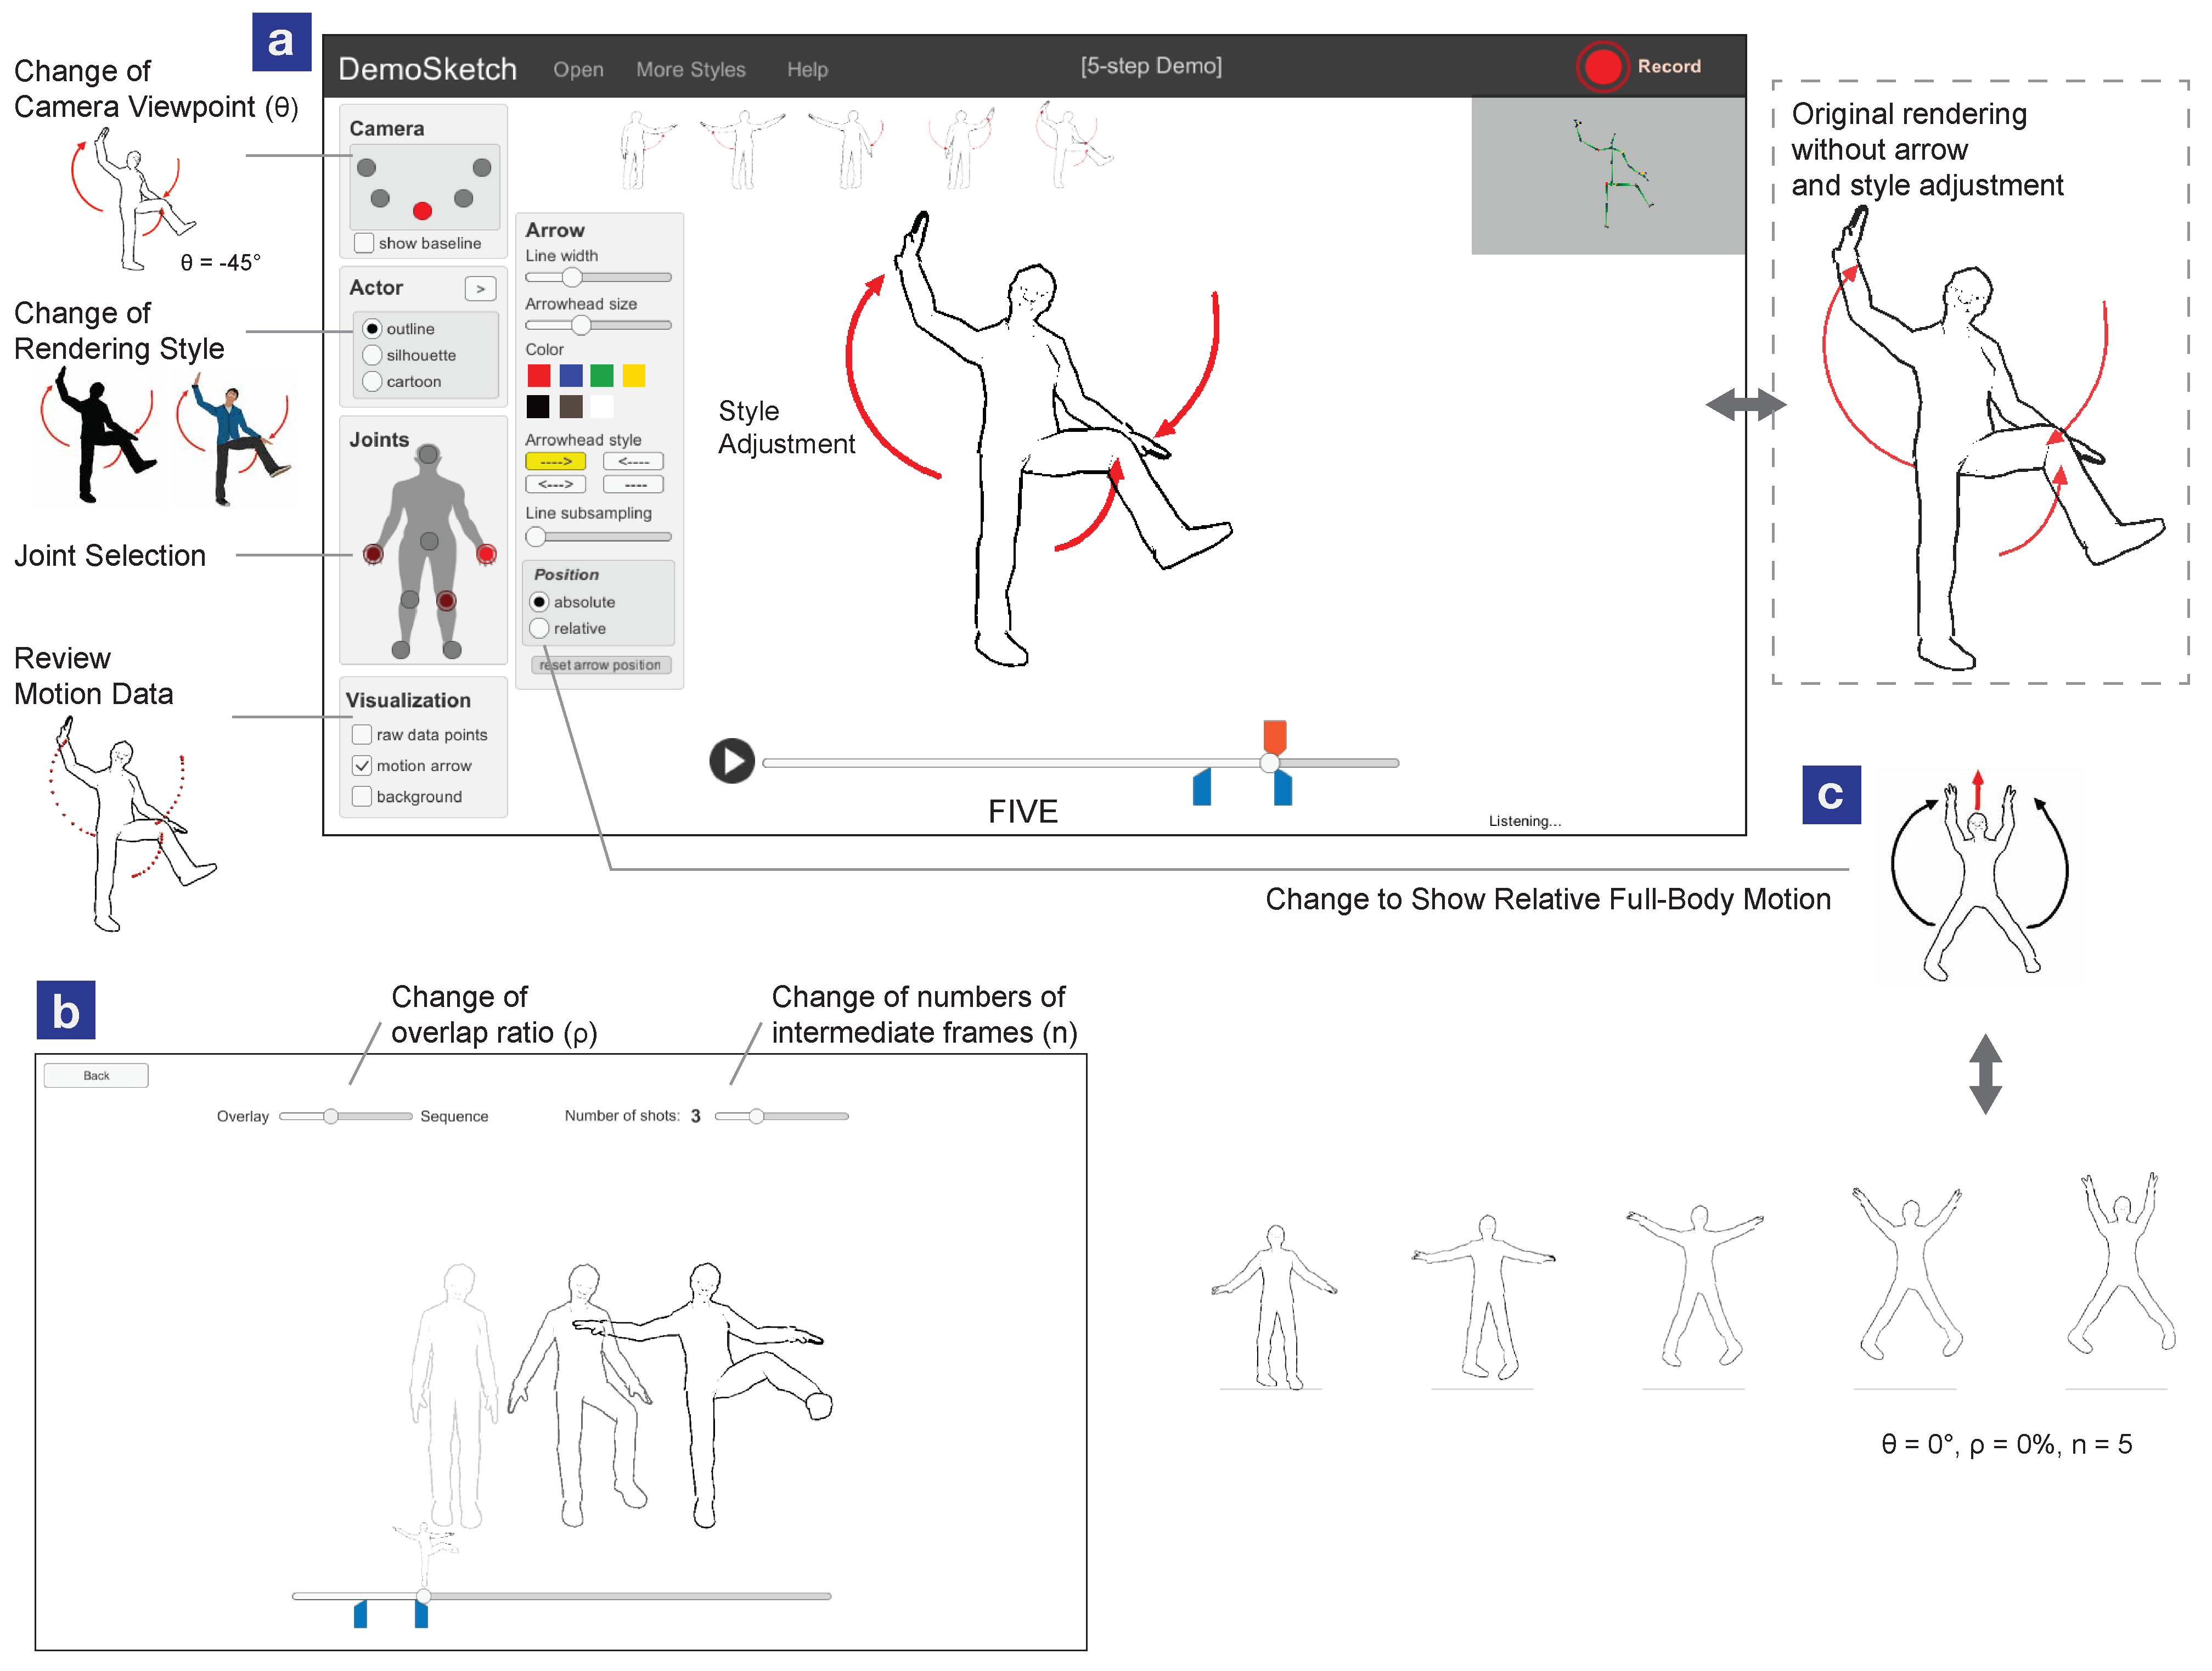
\includegraphics[width=\textwidth]{\demodraw/fig/ui/refinement_ui}
  \caption{Using \systemname{}'s \phaseII{}, the author can refine the visuals (a) and explore more illustration effects (b, c).}
  \label{fig:DemoDrawRefinementUI}
\end{figure*}

\subsubTitleBold{Motion Depiction Adjustments}
Once Marie is satisfied with her demonstration, she walks out of the capture area to her desktop computer. The system automatically switches to the \phaseII{} by revealing post-processing panels in a standard graphical user interface (Figure~\ref{fig:DemoDrawRefinementUI}a).
Using this interface, Marie can adjust several design parameters:
the arrow appearance can be refined, including line width, arrowhead size, and color;
the arrow offset can be adjusted with direct manipulation dragging; %to avoid overlap with the avatar figure
the camera viewpoint can be adjusted by orbiting the camera to a side or three-quarter view;
the joints used for motion paths can be added or removed using a panel;
and the smoothed motion trajectory can be toggled on and off.
%
She could also select a different key pose and adjust the start and end times of a motion segment by dragging the markers on the timeline.
%
In addition, Marie could explore other illustration styles like stroboscopic rendering by selecting numbers of intermediate frames and how they render in one diagram (Figure~\ref{fig:DemoDrawRefinementUI}b).
%
These results can be exported to image files containing the final motion illustrations. %replace vector files - possible but not implemented
